\chapter{Advanced Policies}
After looking at the basics, it is time to dive deeper. Next, we will learn about policies that do not rely on the burst time to function. This means that technically they can be used in a real world application. In reality however, they are usually first modified to fit the environment and the needs better.
We will get to know two subclasses of schedulers: real-time and proportional-share.

\section{Real-Time Scheduling}


The first policy we look at is officially called Multi-Level Feedback Queue, or MLFQ in short. The creator Fernando J. Corbató received a Turning Award for it in 1990. 
As the title already says, this policy tries to predict the future behavior of the processes based on the past.
A job can generally act in two ways:
Either it is a resource-intensive crunching problem (think about exporting a video or compiling code) or it is a program, which needs quick response time (think about your text editor).
In reality most jobs jump between these two states.
We usually want to give the response-focused processes priority, because that is what the user interacts with and it is here that he primarily feels a delay.
The \emph{MLFQ} is used in the Solaris 2.6 Time-Sharing scheduler.
It is part of the time sharing subclass, meaning that it schedules based on an event-driven model, which is usually periodic.

\subsection{Basic Idea}

The policy introduces multiple queues, which each have different priorities.
Each process is assigned to a queue. There are, however, not set in stone.
Based on the reasons above we want to assume that a new process is responsive, because in the worst case scenario, we just need to demote the non-responsive ones.
If however, a process turns out to be interactive, then the user does not feel any lag. 
Each process can run a certain amount of time (also called allotment time) before it is deemed as unworthy of the current priority.
If the allotment is used up, the process gets demoted into a lower queue.

\begin{figure}[h]
    \centering
    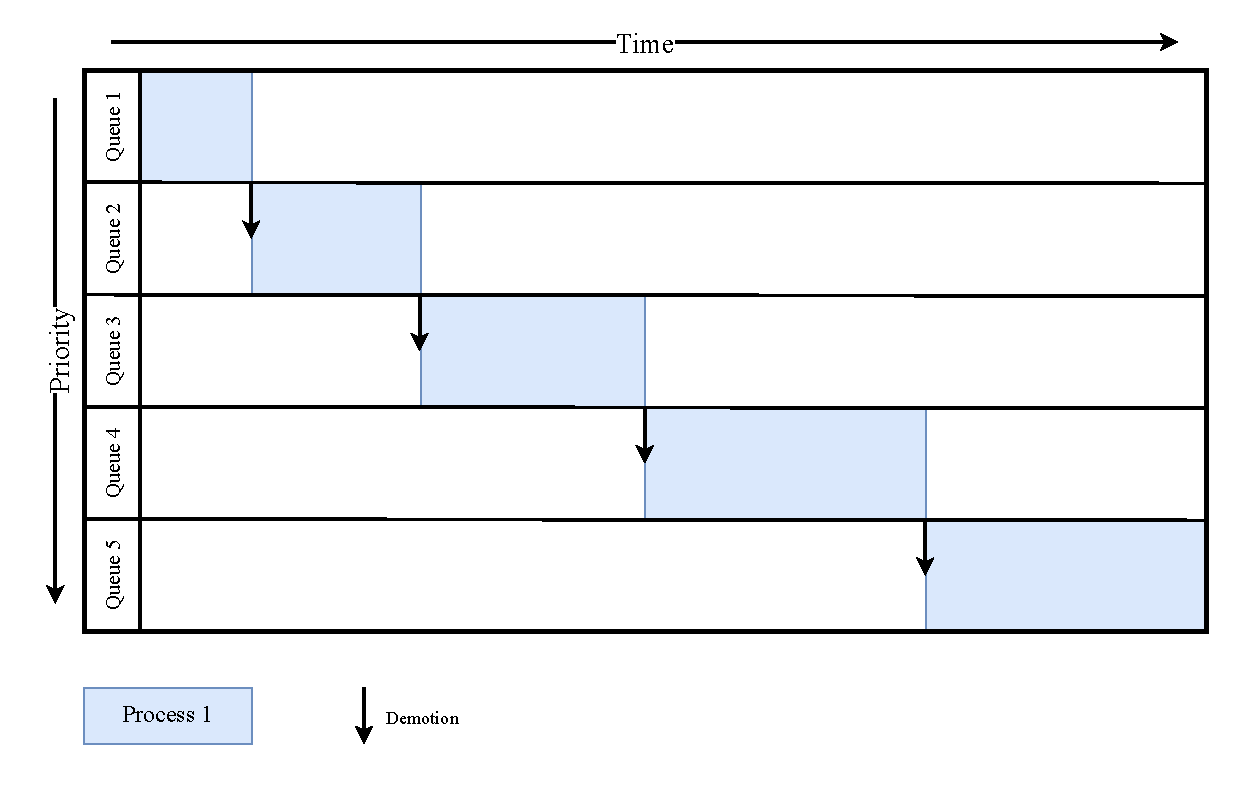
\includegraphics[width=0.8\textwidth]{Assets/MLFQ-Example-1.pdf}
    \caption{Simple working of MLFQ}
    \label{fig:mlfq-example-1}
\end{figure}


As you can see in figure \ref{fig:mlfq-example-1} process one gets demoted after a while.
The lower the queue is, the longer the allotment time. 
This is because we hope that all of the responsive-oriented jobs finish before demoting.
Once these are filtered out we will only have resource heavy tasks left.
These require more time anyways, so the allotment time is stretched out.
After a while the process just ends up at the bottom, at which point it runs until it is finished.
Keep in mind that if the process gets blocked, meaning that it gives up its CPU before the allotment is used up, then they will stay in the same queue and can use up the rest of the allotment before they get demoted. Therefore not the actual time spent in a priority matters but the time spent using the resource.

\subsection{Multiple Processes}

What happens if we introduce another process?
Well, it depends on the priorities. 
Higher priority receives the CPU time.
If they are on the same queue, then they run using \emph{Round Robin} (see section \ref{sec:rr}).


\begin{figure}[h]
    \centering
    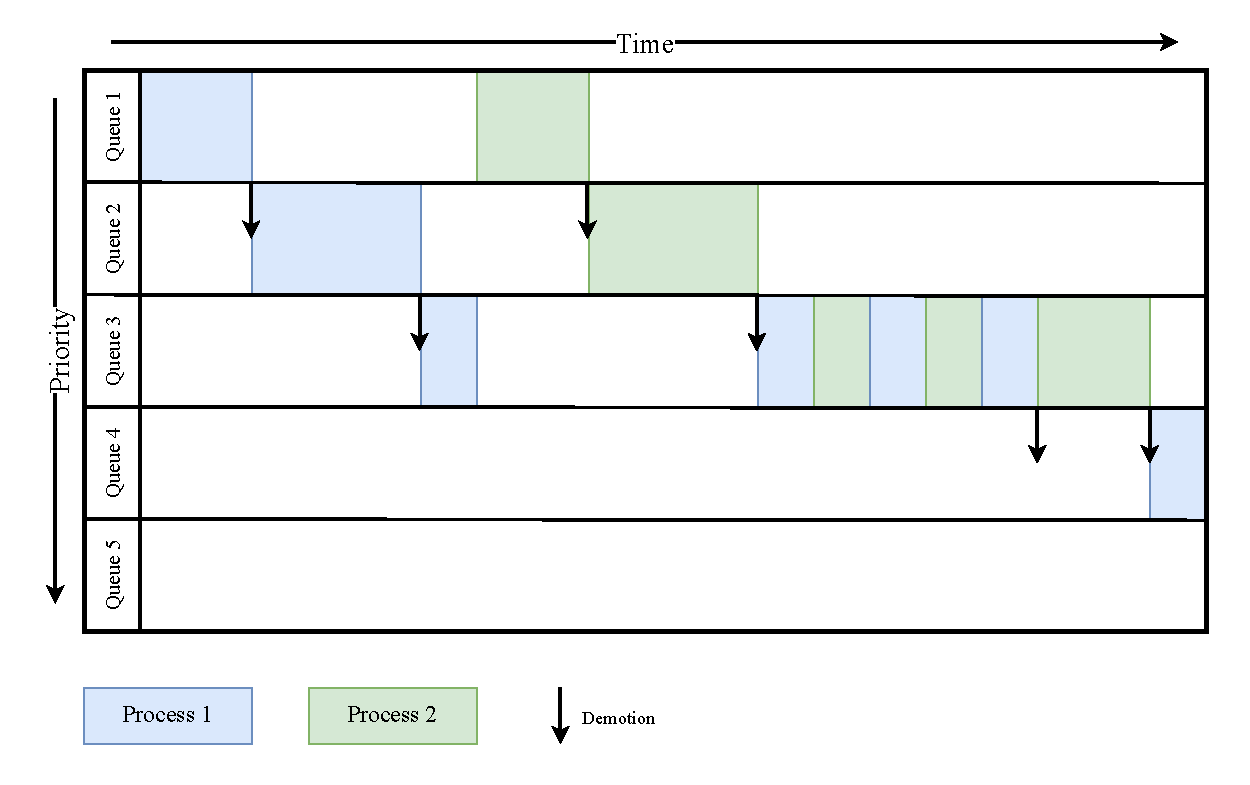
\includegraphics[width=0.8\textwidth]{Assets/MLFQ-Example-2.pdf}
    \caption{Running multiple processes in MLFQ}
    \label{fig:mlfq-example-2}
\end{figure}

As you can see in figure \ref{fig:mlfq-example-2}, once process two is introduced, process one is temporarily starved. The problem is solved once they land on the same queue.
There they run alternately.
Still the more tasks we introduce the more prevalent the starving issue gets.
Take a look at figure \ref{fig:mlfq-example-3} for example. 
Here we have four processes instead of two, which results in process 1 being completely left out.
It could only start running again if processes 2 to 4 either finish or get demoted into priority 5.
That takes quite a lot of time and requires that we don't introduce new tasks during the time waiting.

\begin{figure}[h]
    \centering
    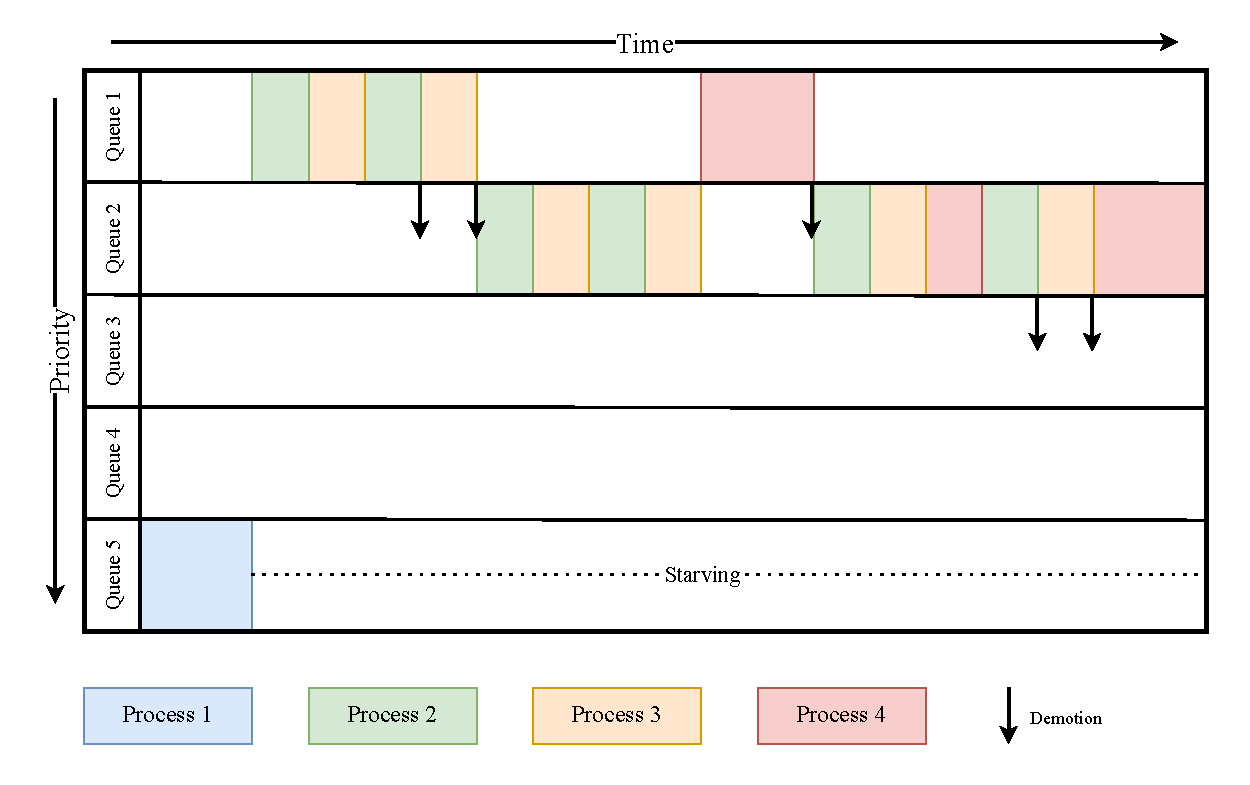
\includegraphics[width=0.8\textwidth]{Assets/MLFQ-Example-3.pdf}
    \caption{Starving Processes in MLFQ}
    \label{fig:mlfq-example-3}
\end{figure}

\subsection{Solving Starvation}

Solving starvation is actually pretty easy.
All we have to do is to make sure that once in a while everybody gets their deserved CPU time.
To do that we introduce a priority boost. All it does is just put every process into priority one every so often.
Even though this introduces another unknown variable that has to be configured, it is just such a crucial element that we have to live with it.

\begin{figure}[h]
    \centering
    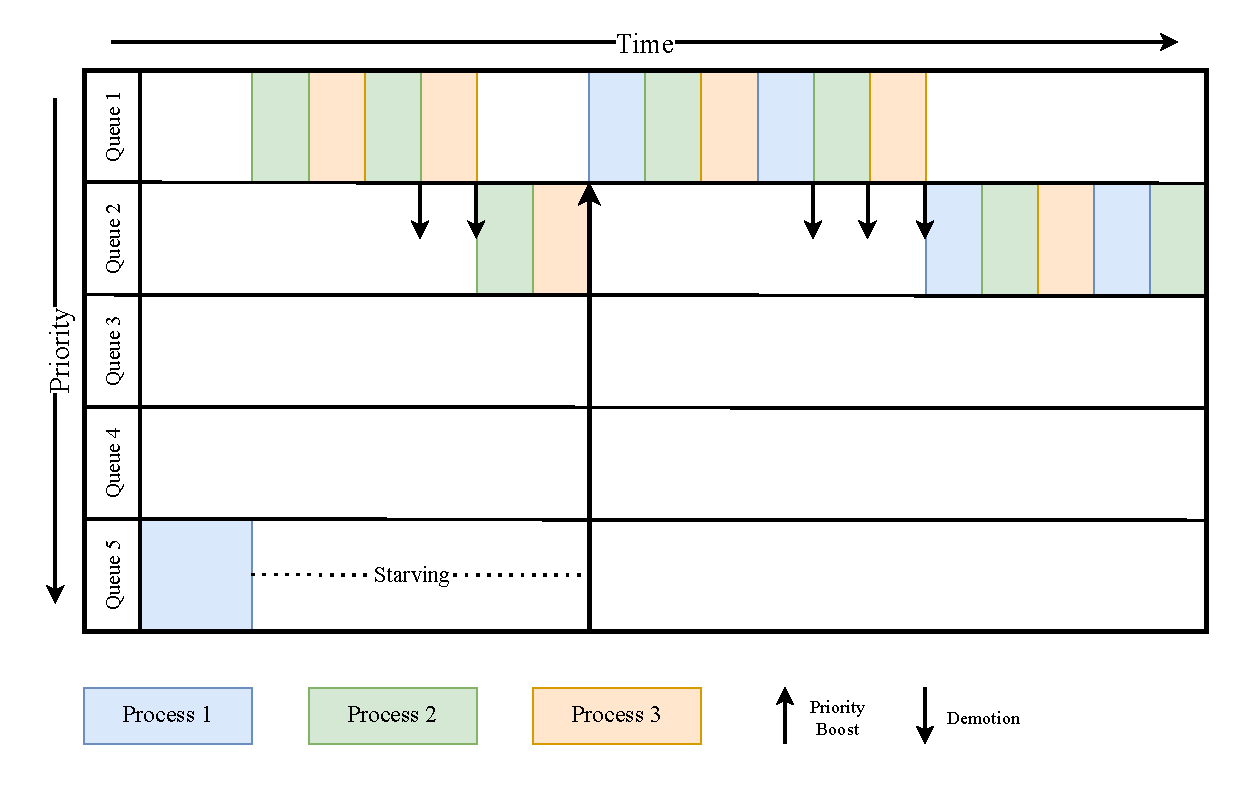
\includegraphics[width=0.8\textwidth]{Assets/MLFQ-Example-4.pdf}
    \caption{Solving Starvation in MLFQ}
    \label{fig:mlfq-example-4}
\end{figure}

\newpage


\subsection{Wrapping Up}

This chapter showed us, how one could approach a scheduling policy that works without needing to know the burst time.
In the end we still end up with many parameters like the allotment time per queue, the number of queues, the quanta for the Round Robin and others.
If used in a real system, the best approach would be to set some sensible defaults and let the administrator adjust the parameters when needed.
To summarize the Multi-Level Feedback Queue, I would like to quote its rules of it from the book OStep \cite{ostep}:
\begin{quote}
\emph{
\begin{enumerate}
        \item If Priority (A) $>$ Priority (B) $\Rightarrow$ A runs and B doesn't
        \item If Priority (A) $=$ Priority (B) $\Rightarrow$ A and B run in Round Robin
        \item When a job enters the system, it is placed at the highest priority
        \item Once a job uses up its time allotment at a given level, its priority is reduced
        \item After some period S, move all the jobs in the system to the topmost queue
\end{enumerate}
}
\end{quote}

\newpage

\section{Proportional-Share Scheduling}

In this chapter we will look at proportional-share scheduling. This type of policy works with weights and assigns them to the processes. For us these weights will take the form of tickets.
Tickets are a form of currency for the computer. Think of it like money.
These can be handed out by the scheduler and give a process the right to use a resource.
Usually, the rigth to a resource is reflected proportianally by the amount of tickets.
Meaning a higher share of tickets will lead to a higher amount of CPU time.
Logically, the response time is inversely proportional. The more tickets you have the less time you have to wait until you run.
These tickets enable easy comparison between processes.
One important difference between money in real life and tickets is that tickets are not consumed when used.
Practically this means that if you buy something you won't lose your bill.
This property leads to the tickets representing the share of the CPU that the job has.
Higher priority processes are weighted more heavily, meaning that they get more tickets

One could imagen these tickets like reservation places in a restaurant. For now it does not matter how the restaurant assigns the places, like it does not matter how the scheduler policy implements the transition from tickets to CPU time. The only thing that is important is that in the end you will have your places and can eat at the restaurant.


\subsection{Operating with Tickets}

You can do two notable things with tickets. First you can transfer them. 
This does exactly what it means. You decrease your amount of tickets and increase someone else's. 
With this you could temporarily boost other processes.
Say, for example, you have a server and a client.
If the client needs something from the server, then it could temporarily boost the servers resources by transfering some of his own tickets.
Of course this requires that the server is trusted or else it could just scam you out of your tickets.
The second way to operate with tickets is ticket inflation and deflation. This can only be done by the owner of the currency and it is only something that we will look at the next section.

\subsection{Ticket Currencies}

Ticket currencies are a way for parent processes to manage their child processes.
Yes, that's right, not all processes are built the same.
A child process is a process that is created by another process.
A parent process is a process, which has at least one child process.
A job can be both a parent and a child at the same time.

The idea behind ticket currencies is that a parent process creates its own unique currency. Therefore he himself can distribute as many bills as he wants. 
However more custom bills does not equal to a higher share of CPU time in the whole system.
Take figure \ref{fig:ticket-currencies} for example. Even though process A had created 100 tickets and gave 40 to process A$_1$ in the end it is all about ratios.
Therefore the overall runtime that A$_1$ has is: 

$$\frac{20\text{T}_\text{G}}{50\text{T}_\text{G}} * \frac{40\text{T}_\text{A}}{100\text{T}_\text{A}} = 0.16 \Rightarrow 16\%$$

There is another hidden benefit. If the parent process receives more global tickets, then if it has a custom currency, there are no further things to do.
If, however, it does not have a custom currency than the process has to transfer these new tickets to the child processes. Overall it can get very messy all too quickly.

\begin{figure}[h]
    \centering
    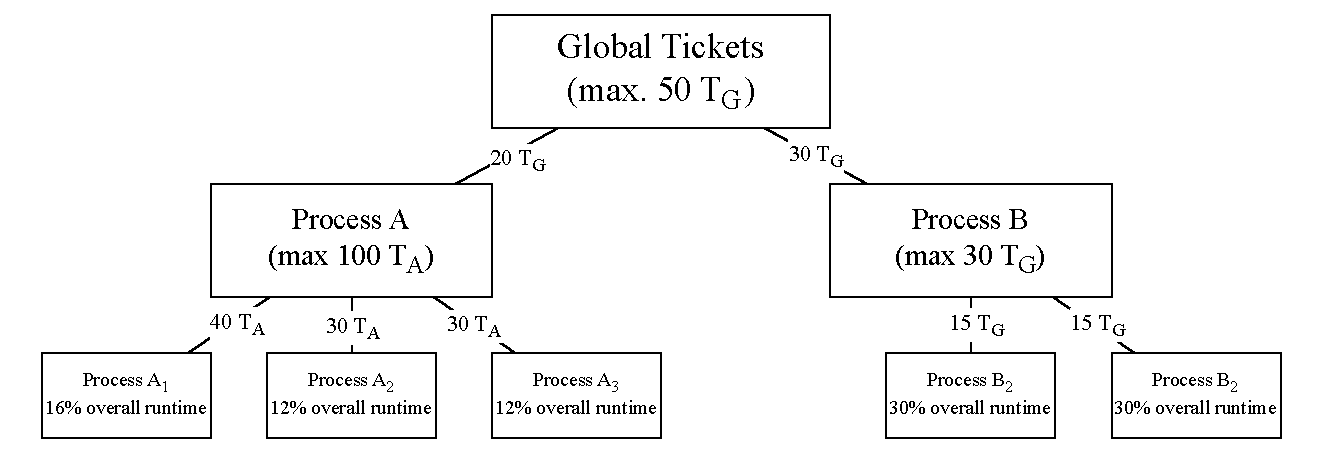
\includegraphics[width=\textwidth]{Assets/Ticket-Currency.pdf}
    \caption{Example of a Custom Ticket Currency}
    \label{fig:ticket-currencies}
\end{figure}
 
Another benefit comes with custom currencies: the ticket inflation or deflation operation.
One needs a custom currency, because it involves creating or destroying tickets. 
Unlike the ticket transfer, ticket inflation does not need a sender and receiver.
A selected process just gets more tickets assigned.
With this the parent process changes the ration of ownership and therefore boosts the selected job.


\subsection{Lottery Scheduling}

Like other things in computer science the name already says a lot. 
Here randomization is exploited to achieve the proportianal share in runtime.
The concept is, that even if over a small scale there will be unavoidable errors, the longer the scheduler runs the more accurate it becomes.
Think of the tickets as lottery tickets.
If the randomization is fair, than the more tickets you have the more you will win.
There is a downside though.
The randomizer algorithm can get pretty expensive.
There is a way to reuse one random seed though, but we will only quickly touch upon it later.
For an example implementation in C take a look at listing \ref{code:lottery-sched}, which is written by Carl A. Waldspurger \cite{waldspurger95}.

\newpage

\begin{figure}[H]
    \begin{minted}[mathescape,
        linenos,
        numbersep=5pt,
        gobble=2,
        frame=lines,
        framesep=2mm,
        ]{cpp}
  typedef struct { /*per-client state */
    ...
    int tickets;
  } *client_t;

  client_t current; /* current resource owner */
  list_t list; /* list of clients competing for resource */
  int global_tickets = 0; /* global ticket sum */

  /* initialize client withspecified allocation */
  void client_init(client_t c, int tickets) {
    c->tickets = tickets; /* initialize client state */ 
    global_tickets += tickets; /* update global sum */
    list_insert(list, c); /* join competition for resource */
  }

  void allocate() {
    int winner, sum;
    client_t c;
    winner = fast_random() % global_tickets; /* randomly select winning ticket */
    /* search list to find client with winning ticket */
    sum = 0;
    for (c = list_first(list);
         c != NULL;
         c = list_next(list, c))
    {
        /* update running sum, stop at winner */
        sum += c->tickets;
        if (sum > winner)
            break;
    }
    current = c;
    use_resource(current); /* grant resource to winner for quantum */
  }
    \end{minted}
    \caption{Implementation of List-Based Lottery Scheduling Algorithm\\Written by: Carl A. Waldspurger \cite{waldspurger95}}
    \label{code:lottery-sched}
\end{figure}

In general implementing dynamic operations is not hard, because the only part that changes is the scheduling part, like choosing a winning ticket.
The clients structure does not need to be modified.
This is because there are no global states. The processes are kept completely isolated from each other and just by looking at the next scheduling you couldn't know how long the scheduler has been running.
In a List-Based system adding and removing clients can be as easy as adding them to the list and adjusting the global max tickets.


\subsubsection{Binary Search}

Even though it is easy to implement, basing the datastructure on a list is quite inefficient, because of the long search time.
Everytime you want to reschedule, you have to create a random number and loop through the list.
However you could use a balanced binary tree to make it much faster.
This is because a list search time scales with n. 
Therefore if you add one more element you will have to search through one more element.
In contrast a binary search scales not with n.
To be more precise it takes $O(log(n))$ to find a specific value.
On average, with each decision we can eliminate half of the remaining candidates.
Therefore overall it is much faster, especially the more values the list contains.

\begin{figure}[h]
    \centering
    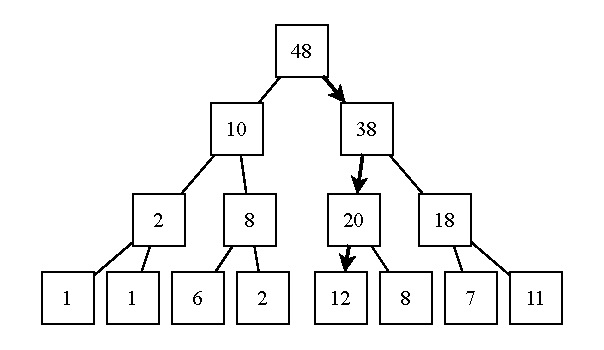
\includegraphics[width=0.8\textwidth]{Assets/Binary-Search.pdf}
    \caption{Binary Search Example}
    \label{fig:binary-search}
\end{figure}

To understand it more, let's go through an example. Let's say there are 48 tickets and our winning one is 20.
To understand the though process better, feel free to look at figure \ref{fig:binary-search}.
For our first decision we need to choose if 20 is above 10 or not.
It is above ten, so we choose the right path.
At this point we have only 38 tickets left and we have to readjust our winning ticket.
We took away 10 tickets from the front so our new winning tickets is 10.
10 is smaller than 20, so we take a left turn and there is no readjusting needed.
In the next step we compare 12 and 10.
12 is larger, which means we take the right path and arrive at our winner process, because 10 is contained in 12.

\subsubsection{Multiwinner Lottery}

Multiwinner Lottery Scheduling is a semi-randomized, semi-deterministic scheduling method.
It is a method to try to minimize the cost of the randomization algorithm.
The basic idea is to reuse the winner.
After you select your winner you take a specific offset to determine the other winners.
One of these lotteries is called a superquantum.

\subsection{Stride Scheduling}

Another approach to implement a proportional-share policy is the so called stride scheduling.
The tickets are used to assign so called strides to the processes.
This stride value will then be used to increment a counter called pass.
The process with the lowest pass value than gets run.

\begin{figure}[h]
    \centering
    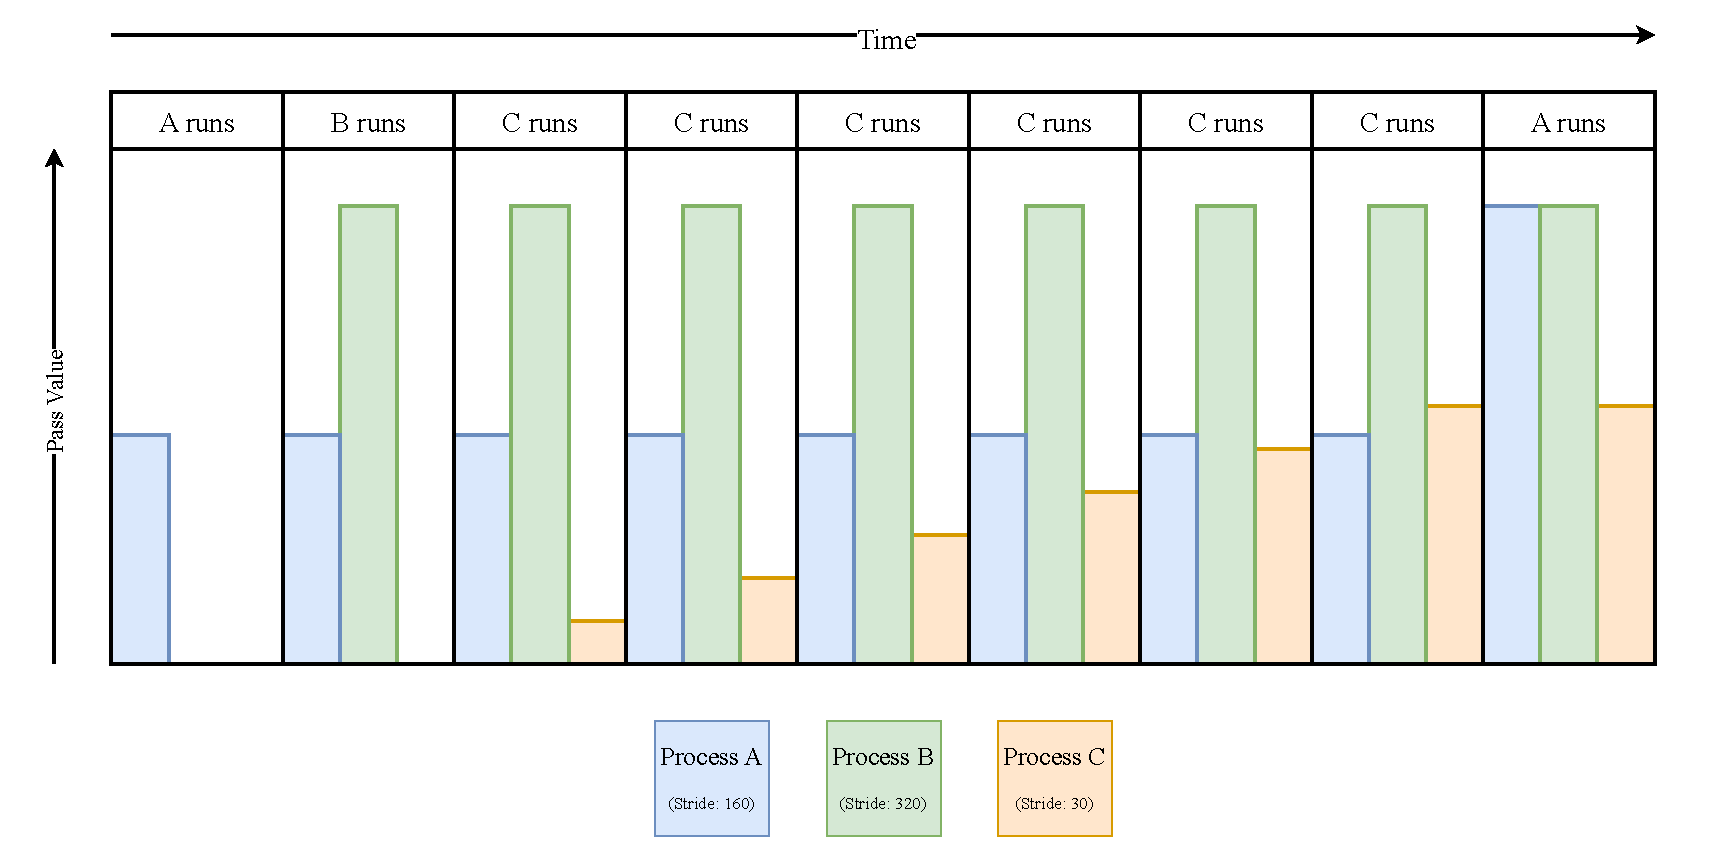
\includegraphics[width=\textwidth]{Assets/Stride-Scheduling.pdf}
    \caption{Stride Scheduling Example}
    \label{fig:stride-scheduling}
\end{figure}

To understand the policy better, let's loot at the example in figure \ref{fig:stride-scheduling}.
We have three processes. Process A has a stride of 160, Process B 320 and Process C has 30. At $t_0$ process A runs. Afterwards its B's turn. C has a much smaller stride, that's why it will have more turns before it catches up to A.
After a while it gets to cyclic pattern.


The benefit of stride scheduling is that one doesn't need a randomizer and the policy itself is much simpler to implement. With such good benefits there comes some disadvantages as well: The processes have global values, meaning that if a new job wants to join, than it has to be adjusted to the current global circumstances. In contrast all you have to do in the lottery is add the assigned tickets to the global maximum tickets.

To solve this, one needs to introduce a constant global pass value, because otherwise the joining processes will monopolize the CPU. 
Look at figure \ref{fig:stride-scheduling} for example.
If a process D joins at the last time interval, than it has to catch up to atleast C. During that time it will have a unreasonable priority over everybody else.
A promised global pass value would eliminate the problem, because one can adjust the entry pass value according to the current situation.
If a task goes into a blocked state or leaves the competition temporarily and than rejoins than its pass value will be global stride plus the stride of the process. The same goes for a brand new job that joins.